% Problem 4.2: Gaussian RNG
% Notes and checklist: ../Exercises/4.02-gaussian-rng/README.md
% Figures:            \includegraphics{4.02-gaussian-rng/figures/<name>}
\exercise{2}{Gaussian RNG}

The CDF of a single Gaussian is the error function, which has no closed-form inverse, so the
method of problem~4.1 does not apply directly. The Box--Muller method avoids this by generating
two Gaussian numbers at once, in polar coordinates \cite{Carlon2025}.

\subsection{The Box--Muller algorithm}

Two independent standard normal numbers $x, y$ have the joint density
$\frac{1}{2\pi} e^{-(x^2+y^2)/2}\,dx\,dy$. In polar coordinates, with $dx\,dy = r\,dr\,d\theta$,
\begin{equation}
  f(r,\theta)\,dr\,d\theta
  = \underbrace{r\,e^{-r^2/2}\,dr}_{r \in [0,\infty)} \; \underbrace{\frac{d\theta}{2\pi}}_{\theta \in [0,2\pi)} .
\end{equation}
The factor $r$ from the Jacobian makes the radial density integrable in closed form:
\begin{equation}
  F(r) = \int_0^r e^{-z^2/2} z\,dz = 1 - e^{-r^2/2}
  \quad\Longrightarrow\quad
  r = \sqrt{-2\ln(1-u_1)}, \qquad \theta = 2\pi u_2 ,
\end{equation}
after which $x = r\cos\theta$ and $y = r\sin\theta$. Because the density factorises in $r$ and
$\theta$, the two must be drawn from two \emph{independent} uniform numbers $u_1, u_2$. Using the same
$u$ for both makes $r$ a function of $\theta$, and all points lie on one spiral; this was a bug
in a first version of the code.

The density also factorises in Cartesian coordinates, $\frac{1}{2\pi}e^{-(x^2+y^2)/2} = \phi(x)\,\phi(y)$
with $\phi$ the standard normal density. So $x$ and $y$ are not only normal but independent.

\begin{figure}[htbp]
  \centering
  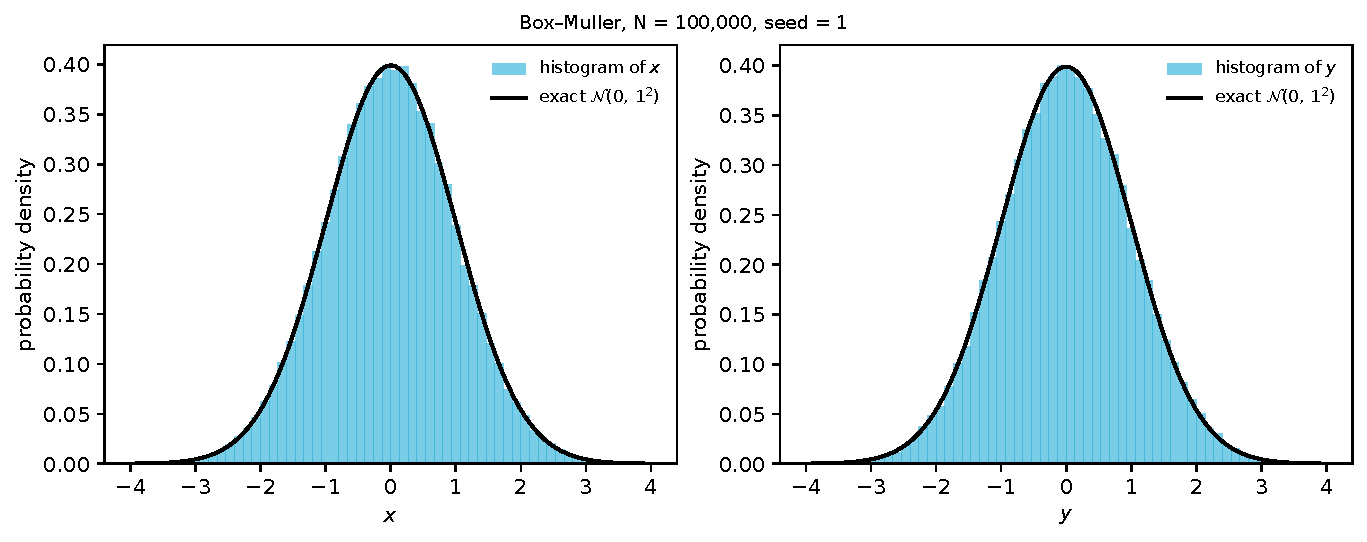
\includegraphics[width=0.9\linewidth]{4.02-gaussian-rng/figures/box_muller_hist}
  \caption{Box--Muller: histograms (60 bins) of $x$ and $y$ from $N = 10^5$ pairs, with the exact
    $\mathcal N(0,1)$ density. Seed 1.}
  \label{fig:4.2-hist}
\end{figure}

\begin{table}[htbp]
  \centering
  \caption{Sample moments of $N = 10^5$ Box--Muller pairs (seed 1). The error on the mean is
    $s/\sqrt N$. For (b) the same pairs are rescaled.}
  \label{tab:4.2-moments}
  \begin{tabular}{llcc}
    \toprule
    case & variable & mean & variance \\
    \midrule
    (a) $\mathcal N(0,1)$             & $x$  & $-0.0033 \pm 0.0032$ & $0.995$ \\
                                      & $y$  & $+0.0072 \pm 0.0032$ & $1.004$ \\
    (b) $\mu = 3$, $\sigma = 2$       & $x'$ & $2.9934 \pm 0.0063$  & $3.981$ \\
                                      & $y'$ & $3.0145 \pm 0.0063$  & $4.014$ \\
    (b) $\boldsymbol\mu = (3,-5)$, $\boldsymbol\sigma = (2,1)$
                                      & $x'$ & $2.9934 \pm 0.0063$  & $3.981$ \\
                                      & $y'$ & $-4.9928 \pm 0.0032$ & $1.004$ \\
    \bottomrule
  \end{tabular}
\end{table}

Figure~\ref{fig:4.2-hist} shows that both coordinates follow the standard normal density, and
table~\ref{tab:4.2-moments} gives means compatible with 0 and variances compatible with 1 (the
relative error on a variance from $10^5$ points is $\sqrt{2/N} \approx 0.45\,\%$). The mean of $y$ is
2.2 standard errors from zero, which is an ordinary fluctuation for one seed. The scatter plot of
figure~\ref{fig:4.2-xy} (left) is a circularly symmetric cloud, and the correlation coefficient
$\rho_{xy} = -0.0016$ is compatible with $0 \pm 1/\sqrt N = 0 \pm 0.0032$. A zero correlation alone
does not prove independence; the factorisation of the density above does.

\subsection{Mean $\mu$ and variance $\sigma^2$}

The algorithm does not need to change: the output is rescaled,
\begin{equation}
  x' = \mu + \sigma x, \qquad y' = \mu + \sigma y .
\end{equation}
Then $\avg{x'} = \mu$ and $\mathrm{Var}(x') = \sigma^2\,\mathrm{Var}(x) = \sigma^2$. The density stays
Gaussian, because the change of variables $x = (x'-\mu)/\sigma$, $dx = dx'/\sigma$ gives
$\frac{1}{\sqrt{2\pi\sigma^2}} e^{-(x'-\mu)^2/2\sigma^2}$. Equivalently, one can draw
$r = \sigma\sqrt{-2\ln(1-u_1)}$ and shift the result by $\mu$.

\kulbox[5pt]{Box--Muller: $r = \sqrt{-2\ln(1-u_1)}$, $\theta = 2\pi u_2$, then
$x = \mu + \sigma r\cos\theta$ and $y = \mu + \sigma r\sin\theta$ are two independent
$\mathcal N(\mu,\sigma^2)$ numbers.}

We tested this with $\mu = 3$, $\sigma = 2$ for both coordinates, and with different parameters per
axis, $\boldsymbol\mu = (3,-5)$ and $\boldsymbol\sigma = (2,1)$. The moments in
table~\ref{tab:4.2-moments} agree with the targets. They are the same Box--Muller pairs as in (a), so the
relative deviations are those of (a). With different $\sigma$ per axis the cloud becomes an ellipse
elongated along $x$ (figure~\ref{fig:4.2-xy}, right).

\begin{figure}[htbp]
  \centering
  \begin{subfigure}{0.46\linewidth}
    \centering
    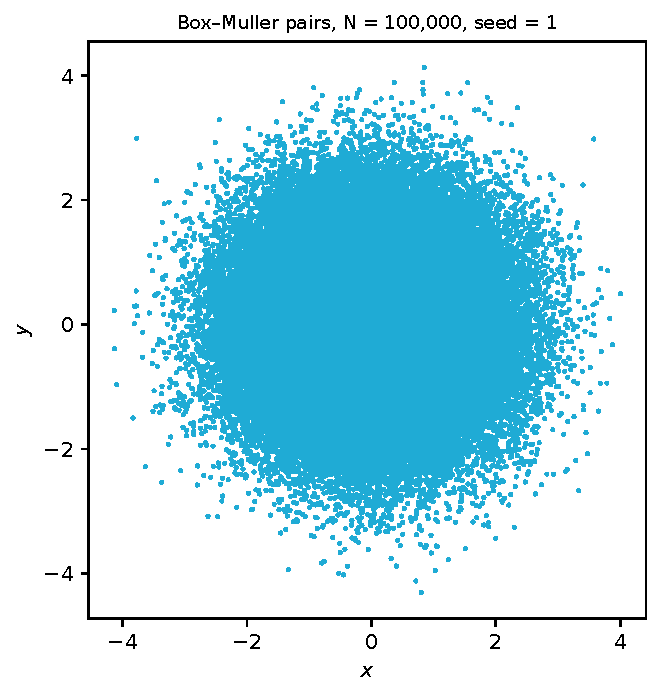
\includegraphics[width=\linewidth]{4.02-gaussian-rng/figures/box_muller_xy}
    \caption{$\mathcal N(0,1)$ for both coordinates.}
  \end{subfigure}\hfill
  \begin{subfigure}{0.46\linewidth}
    \centering
    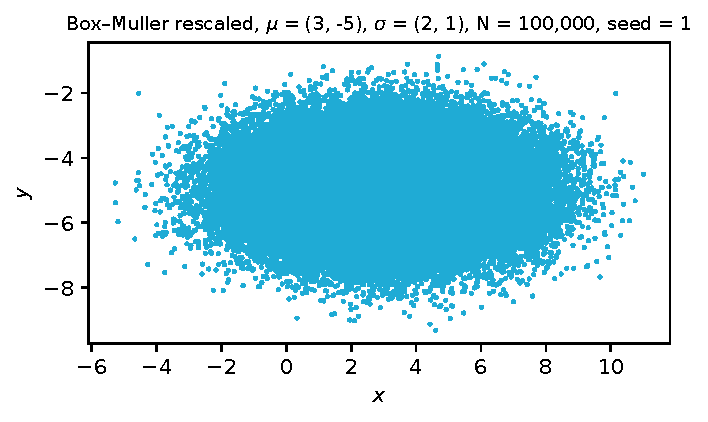
\includegraphics[width=\linewidth]{4.02-gaussian-rng/figures/box_muller_xy_mu_sigma_asym}
    \caption{$\boldsymbol\mu = (3,-5)$, $\boldsymbol\sigma = (2,1)$.}
  \end{subfigure}
  \caption{Scatter plots of $N = 10^5$ Box--Muller pairs $(x,y)$, seed 1. The rescaled pairs on the
    right are the same as on the left, shifted by $\boldsymbol\mu$ and stretched by $\boldsymbol\sigma$.}
  \label{fig:4.2-xy}
\end{figure}
